\documentclass[12pt]{article}
\usepackage[margin=1.0in]{geometry}
\usepackage{setspace}
\usepackage{titling}

\usepackage{amsmath,amsthm,amssymb}
\usepackage{graphicx}
\usepackage{enumerate}
\usepackage[shortlabels]{enumitem}

\setstretch{1.5}
\setlength{\droptitle}{-8em}

\usepackage{/home/sabbir/texmf/longdivision}
\usepackage{/home/sabbir/texmf/karnaugh-map}

\begin{document}

  \title{605.611 - Foundations of Computer Architecture \\ Assignment 02\vspace{-0.5em}}
  \author{Sabbir Ahmed}
  \maketitle
  \vspace{-1em}

  \begin{enumerate}

    % 1
    \item Convert the following fixed point numbers to binary fixed point. Give both the actual values, and normalize the values so that they have a binary 1 as the value for the left of the decimal point.
    \begin{enumerate}
      \item 7.25

      \textbf{Answer:}
      Integral part: 7 = $(0111)_2$ \\
      Repeatedly multiplying the fractional part by 2:
      \begin{align*}
        & 0.25 \\
        &\begin{tabular}{ccccc}
          & 0 & . & 2 & 5 \\
        $\times$ &  &  &  & 2 \\
        \hline
          & 0 & . & 5 & 0 \\
        $\times$ &  &  &  & 2 \\
        \hline
          & 1 & . & 0 & 0 \\
        \end{tabular} \\
        &= (10)_2 \\
        &\Rightarrow 7.25 = (111.01)_2, \text{(normalized to} \ (1.1101)_2 \times 2^{2})
      \end{align*}

      \item 13.5

      \textbf{Answer:}
      Integral part: 13 = $(1101)_2$ \\
      Repeatedly multiplying the fractional part by 2:
      \begin{align*}
        & 0.50 \\
        &\begin{tabular}{ccccc}
          & 0 & . & 5 & 0 \\
        $\times$ &  &  &  & 2 \\
        \hline
          & 1 & . & 0 & 0 \\
        \end{tabular} \\
        &= (1)_2 \\
        &\Rightarrow 13.5 = (1101.1)_2, \text{(normalized to} \ (1.1011)_2 \times 2^{3})
      \end{align*}

      \item 0.5625

      \textbf{Answer:}
      Integral part: 0 \\
      Repeatedly multiplying the fractional part by 2:
      \begin{align*}
        & 0.5625 \\
        &\begin{tabular}{ccccccc}
          & 0 & . & 5 & 6 & 2 & 5 \\
        $\times$ & & & & & & 2 \\
        \hline
          & 1 & . & 1 & 2 & 5 & 0 \\
        $\times$ & & & & & & 2 \\
        \hline
          & 0 & . & 2 & 5 & 0 & 0 \\
        $\times$ & & & & & & 2 \\
        \hline
          & 0 & . & 5 & 0 & 0 & 0 \\
        $\times$ & & & & & & 2 \\
        \hline
          & 1 & . & 0 & 0 & 0 & 0 \\
        \end{tabular} \\
        &= (1001)_2 \\
        &\Rightarrow 0.5625 = (0.1001)_2, \text{(normalized to} \ (1.001)_2 \times 2^{-1})
      \end{align*}

      \item 0.125

      \textbf{Answer:}
      Integral part: 0 \\
      Repeatedly multiplying the fractional part by 2:
      \begin{align*}
        & 0.125 \\
        &\begin{tabular}{cccccc}
          & 0 & . & 1 & 2 & 5 \\
        $\times$ & & & & & 2 \\
        \hline
          & 0 & . & 2 & 5 & 0 \\
        $\times$ & & & & & 2 \\
        \hline
          & 0 & . & 5 & 0 & 0 \\
        $\times$ & & & & & 2 \\
        \hline
          & 1 & . & 0 & 0 & 0 \\
        \end{tabular} \\
        &= (001)_2 \\
        &\Rightarrow 0.5625 = (0.001)_2, \text{(normalized to} \ (1.0)_2 \times 2^{-3})
      \end{align*}

      \item 127.625

      \textbf{Answer:}
      Integral part: 127 = $(0111 1111)$ \\
      Repeatedly multiplying the fractional part by 2:
      \begin{align*}
        & 0.625 \\
        &\begin{tabular}{cccccc}
          & 0 & . & 6 & 2 & 5 \\
        $\times$ & & & & & 2 \\
        \hline
          & 1 & . & 2 & 5 & 0 \\
        $\times$ & & & & & 2 \\
        \hline
          & 0 & . & 5 & 0 & 0 \\
        $\times$ & & & & & 2 \\
        \hline
          & 1 & . & 0 & 0 & 0 \\
        \end{tabular} \\
        &= (101)_2 \\
        &\Rightarrow 127.625 = (1111111.101)_2, \text{(normalized to} \ (1.111111101)_2 \times 2^{6})
      \end{align*}

      \item 51,025.025

      \textbf{Answer:}
      Integral part: 51025 =
      \begin{align*}
        &\Rightarrow 51025 \\
        &= \intlongdivision{51025}{2}\quad
        \intlongdivision{25512}{2}\quad
        \intlongdivision{12756}{2}\quad
        \intlongdivision{6378}{2}\quad
        \intlongdivision{3189}{2}\quad
        \intlongdivision{1594}{2}\\
        &\intlongdivision{797}{2}\quad
        \intlongdivision{398}{2}\quad
        \intlongdivision{199}{2}\quad
        \intlongdivision{99}{2}\quad
        \intlongdivision{49}{2}\quad
        \intlongdivision{24}{2}\quad
        \intlongdivision{12}{2}\quad
        \intlongdivision{6}{2}\\
        &\intlongdivision{3}{2}\quad
        \intlongdivision{1}{2}\\
        &\Rightarrow (1100 \ 0111 \ 0101 \ 0001)_2
      \end{align*}
      Repeatedly multiplying the fractional part by 2:
      \begin{align*}
        & 0.025 \\
        &\begin{tabular}{cccccc}
          & 0 & . & 0 & 2 & 5 \\
        $\times$ & & & & & 2 \\
        \hline
          & 0 & . & 0 & 5 & 0 \\
        $\times$ & & & & & 2 \\
        \hline
          & 0 & . & 1 & 0 & 0 \\
        $\times$ & & & & & 2 \\
        \hline
          & 0 & . & 2 & 0 & 0 \\
        $\times$ & & & & & 2 \\
        \hline
          & 0 & . & 4 & 0 & 0 \\
        $\times$ & & & & & 2 \\
        \hline
          & 0 & . & 8 & 0 & 0 \\
        $\times$ & & & & & 2 \\
        \hline
          & 1 & . & 6 & 0 & 0 \\
        $\times$ & & & & & 2 \\
        \hline
          & 1 & . & 2 & 0 & 0 \\
        $\times$ & & & & & 2 \\
        \hline
          & 0 & . & 4 & 0 & 0 \\
        $\times$ & & & & & 2 \\
        \hline
          & 0 & . & 8 & 0 & 0 \\
        $\times$ & & & 2 \\
        \hline
          & 1 & . & 6 & 0 & 0 \\
        $\times$ & & & & & 2 \\
        \hline
          & 1 & . & 2 & 0 & 0 \\
        \end{tabular} \\
        &\text{The pattern $(0000011)_2$ appears to keep repeating}  \\
        &\Rightarrow 51,025.025 = (1100011101010001.0000011)_2, \\
        &\text{(normalized to} \ (1.1000111010100010000011)_2 \times 2^{15})
      \end{align*}

      \item 7.1

      \textbf{Answer:}
      Integral part: 7 = $(111)_2$ \\
      Repeatedly multiplying the fractional part by 2:
      \begin{align*}
        & 0.1 \\
        &\begin{tabular}{cccc}
          & 0 & . & 1 \\
        $\times$ & & & 2 \\
        \hline
          & 0 & . & 2 \\
        $\times$ & & & 2 \\
        \hline
          & 0 & . & 4 \\
        $\times$ & & & 2 \\
        \hline
          & 0 & . & 8 \\
        $\times$ & & & 2 \\
        \hline
          & 1 & . & 6 \\
        $\times$ & & & 2 \\
        \hline
          & 1 & . & 2 \\
        $\times$ & & & 2 \\
        \hline
          & 0 & . & 4 \\
        $\times$ & & & 2 \\
        \hline
          & 0 & . & 8 \\
        $\times$ & & & 2 \\
        \hline
          & 1 & . & 6 \\
        $\times$ & & & 2 \\
        \hline
          & 1 & . & 2 \\
        \end{tabular} \\
        &\text{The pattern $(0011)_2$ appears to keep repeating}  \\
        &\Rightarrow 7.1 = (111.0\overline{00110011})_2, \\
        &\text{(normalized to} \ (1.110\overline{00110011})_2 \times 2^{2})
      \end{align*}

      \item 5.2

      \textbf{Answer:}
      Integral part: 5 = $(101)_2$ \\
      Repeatedly multiplying the fractional part by 2:
      \begin{align*}
        & 0.2 \\
        &\begin{tabular}{cccc}
          & 0 & . & 2 \\
        $\times$ & & & 2 \\
        \hline
          & 0 & . & 4 \\
        $\times$ & & & 2 \\
        \hline
          & 0 & . & 8 \\
        $\times$ & & & 2 \\
        \hline
          & 1 & . & 6 \\
        $\times$ & & & 2 \\
        \hline
          & 1 & . & 2 \\
        $\times$ & & & 2 \\
        \hline
          & 0 & . & 4 \\
        $\times$ & & & 2 \\
        \hline
          & 0 & . & 8 \\
        $\times$ & & & 2 \\
        \hline
          & 1 & . & 6 \\
        \end{tabular} \\
        &\text{The pattern $(0011)_2$ appears to keep repeating}  \\
        &\Rightarrow 7.1 = (101.\overline{00110011})_2, \\
        &\text{(normalized to} \ (1.01\overline{00110011})_2 \times 2^{2})
      \end{align*}

    \end{enumerate}

    % 5
    \setcounter{enumi}{4}
    \item Convert the following from decimal to excess 127 format. Write your answers as hexadecimal digits.
    \begin{enumerate}
      \item -4

      \textbf{Answer:}
      \begin{align*}
        &-4 + 127 \\
        &= 123 = 7B_{16}
      \end{align*}

      \item 4

      \textbf{Answer:}
      \begin{align*}
        &4 + 127 \\
        &= 131 = 83_{16}
      \end{align*}

      \setcounter{enumii}{3}
      \item 7

      \textbf{Answer:}
      \begin{align*}
        &7 + 127 \\
        &= 134 = 86_{16}
      \end{align*}

      \item -7

      \textbf{Answer:}
      \begin{align*}
        &-7 + 127 \\
        &= 120 = 78_{16}
      \end{align*}

    \end{enumerate}

    % 8
    \setcounter{enumi}{7}
    \item Single precision floating point numbers have 7 digit decimal precision and double floating point numbers have 15 digit precision. Explain how these precision values are arrived at, and what they mean.

    Single and double precision floating point numbers are represented by 32 and 64 bits respectively. Single precision floats allocates 1 bit for the sign and 8 bits for the exponent, leaving the remaining 23 bits to represent the mantissa. The largest 23-bit decimal is $2^{23}-1=8,388,607$ which is a 7 digit decimal. Similarly, double precision floats allocate 52 bits to represent the mantissa with the largest decimal being $2^{52}-1$. To find the number of digits in this large decimal, we can compute $\log_{10}(2^{52})=52\cdot \log_{10}(2)$ which approximates to 15.65 decimals.

    % 9
    \item Convert the following numbers to IEEE 754 single precision numbers. Give your answers as hexadecimal numbers (do not give me binary, I cannot read it accurately. I WILL misread it and you WILL lose points).
    \begin{enumerate}
      \item 7.25

      \textbf{Answer:}
      Since the decimal is positive, the sign bit is 0 \\
      $7.25 = (1.1101)_2 \times 2^{2} \ \text{from Part 1a}$ \\
      Mantissa: $(1101)_2$ \\
      Exponent: $+2 \Rightarrow 2 + 127 = (1000 \ 0001)_2$ \\
      Therefore,
      \begin{align*}
        &\Rightarrow (0100 \ 0000 \ 1110 \ 1000)_2 \\
        &= (40E8 \ 0000)_{16}
      \end{align*}

      \item 13.5

      \textbf{Answer:}
      Since the decimal is positive, the sign bit is 0 \\
      $13.5 = (1.1011)_2 \times 2^{3} \ \text{from Part 1b}$ \\
      Mantissa: $(1011)_2$ \\
      Exponent: $+3 \Rightarrow 3 + 127 = (1000 \ 0010)_2$ \\
      Therefore,
      \begin{align*}
        &\Rightarrow (0100 \ 0001 \ 0101 \ 1000)_2 \\
        &= (4158 \ 0000)_{16}
      \end{align*}

      \item 0.5625

      \textbf{Answer:}
      Since the decimal is positive, the sign bit is 0 \\
      $0.5625 = (1.001)_2 \times 2^{-1} \ \text{from Part 1c}$ \\
      Mantissa: $(001)_2$ \\
      Exponent: $-1 \Rightarrow -1 + 127 = (0111 \ 1110)_2$ \\
      Therefore,
      \begin{align*}
        &\Rightarrow (0011 \ 1111 \ 0001 \ 0000)_2 \\
        &= (3F10 \ 0000)_{16}
      \end{align*}

      \item 0.125

      \textbf{Answer:}
      Since the decimal is positive, the sign bit is 0 \\
      $0.125 = (1.0)_2 \times 2^{-3} \ \text{from Part 1d}$ \\
      Mantissa: 0 \\
      Exponent: $-3 \Rightarrow -3 + 127 = (0111 \ 1100)_2$ \\
      Therefore,
      \begin{align*}
        &\Rightarrow (0011 \ 1110 \ 0000 \ 0000)_2 \\
        &= (3E00 \ 0000)_{16}
      \end{align*}

      \item 127.625

      \textbf{Answer:}
      Since the decimal is positive, the sign bit is 0 \\
      $127.625 = (1.111111101)_2 \times 2^{6} \ \text{from Part 1e}$ \\
      Mantissa: $(111111101)_2$ \\
      Exponent: $6 \Rightarrow 6 + 127 = (1000 \ 0101)_2$ \\
      Therefore,
      \begin{align*}
        &\Rightarrow (0100 \ 0010 \ 1111 \ 1111 \ 0100)_2 \\
        &= (42FF \ 4000)_{16}
      \end{align*}

      \item 51025.025

      \textbf{Answer:}
      Since the decimal is positive, the sign bit is 0 \\
      $51025.025 = (1.1000111010100010000011)_2 \times 2^{15} \ \text{from Part 1f}$ \\
      Mantissa: $(1000111010100010000011)_2$ \\
      Exponent: $15 \Rightarrow 15 + 127 = (1000 \ 1110)_2$ \\
      Therefore,
      \begin{align*}
        &\Rightarrow (0100 \ 0111 \ 0100 \ 0111 \ 0101 \ 0001 \ 0000 \ 0110)_2 \\
        &= (4747 \ 5106)_{16}
      \end{align*}

    \end{enumerate}

    % 10
    \item For each of the following truth tables:
    \begin{itemize}
      \item Give the DNF equation for the table.
      \item Give the minimal equation.
      \item Using Boolean algebra show the two Boolean equations are equivalent.
      \item Draw the circuit in Logisim. Be prepared to draw the circuit by hand.
    \end{itemize}

    \begin{enumerate}
      \item
      \noindent
      $\displaystyle
      \left[
        \begin{array}{c c c|c}
          \textbf{A} & \textbf{B} & \textbf{C} & \textbf{f(A,B,C)} \\
          \hline
          0 & 0 & 0 & 0 \\
          0 & 0 & 1 & 1 \\
          0 & 1 & 0 & 1 \\
          0 & 1 & 1 & 0 \\
          1 & 0 & 0 & 0 \\
          1 & 0 & 1 & 1 \\
          1 & 1 & 0 & 1 \\
          1 & 1 & 1 & 0
        \end{array}
      \right]$

      \vspace{2em}
      \textbf{Answer:}
      \begin{Karnaughvuit}
        \maxterms{0,3,4,7}
        \minterms{1,2,5,6}
        \implicant{1}{5}{green}
        \implicant{2}{6}{red}
      \end{Karnaughvuit}

      DNF: $\overline{A}\overline{B}C + \overline{A}B\overline{C} + A\overline{B}C + AB\overline{C}$

      Minimal equation: $\overline{B}C + B\overline{C}$

      Show $\overline{A}\overline{B}C + \overline{A}B\overline{C} + A\overline{B}C + AB\overline{C} = \overline{B}C + B\overline{C}$
      \begin{align*}
        \overline{A}\overline{B}C + \overline{A}B\overline{C} + A\overline{B}C + AB\overline{C} &= \overline{A}(\overline{B}C + B\overline{C}) + A(\overline{B}C + B\overline{C}) \\
        &= (\overline{A}+A)(\overline{B}C + B\overline{C})\\
        &=(1)(\overline{B}C + B\overline{C})\\
        &=\overline{B}C + B\overline{C}
      \end{align*}

      \begin{figure}[h]
        \centering
        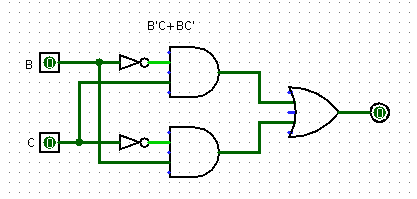
\includegraphics[width=0.8\textwidth]{assn/02/media/10a.png}
        \caption{Circuit Diagram of the Truth Table 10a in Logisim}
      \end{figure}
      % \clearpage

      \item
      \noindent
      $\displaystyle
      \left[
        \begin{array}{c c c|c}
          \textbf{A} & \textbf{B} & \textbf{C} & \textbf{f(A,B,C)} \\
          \hline
          0 & 0 & 0 & 1 \\
          0 & 0 & 1 & 1 \\
          0 & 1 & 0 & 1 \\
          0 & 1 & 1 & 1 \\
          1 & 0 & 0 & 0 \\
          1 & 0 & 1 & 1 \\
          1 & 1 & 0 & 0 \\
          1 & 1 & 1 & 1
        \end{array}
      \right]$

      \vspace{2em}
      \textbf{Answer:}
      \begin{Karnaughvuit}
        \maxterms{4,6}
        \minterms{0,1,2,3,5,7}
        \implicant{0}{2}{green}
        \implicant{1}{7}{red}
      \end{Karnaughvuit}

      DNF: $\overline{A}\overline{B}\overline{C} + \overline{A}\overline{B}C + \overline{A}BC + \overline{A}B\overline{C} + \overline{A}\overline{B}C + A\overline{B}C + \overline{A}BC + ABC$

      Minimal equation: $\overline{A} + C$

      Show $\overline{A}\overline{B}\overline{C} + \overline{A}\overline{B}C + \overline{A}BC + \overline{A}B\overline{C} + \overline{A}\overline{B}C + A\overline{B}C + \overline{A}BC + ABC = \overline{A} + C$
      \begin{align*}
        &\overline{A}\overline{B}\overline{C} + \overline{A}\overline{B}C + \overline{A}BC + \overline{A}B\overline{C} + \overline{A}\overline{B}C + A\overline{B}C + \overline{A}BC + ABC\\
        &= \overline{A}\overline{B}\overline{C} + \overline{A}\overline{B}C + \overline{A}BC + \overline{A}B\overline{C} + A\overline{B}C + ABC \\
        &= \overline{A}(\overline{B}\overline{C} + \overline{B}C + BC + B\overline{C}) + AC(\overline{B} + B) \\
        &= \overline{A}(\overline{B} + \overline{C} + BC + \overline{B}C + B\overline{C}) + AC(1) \\
        &= \overline{A}(\overline{B} + \overline{B}C + \overline{C} + B\overline{C} + BC) + AC \\
        &= \overline{A}(\overline{B} + \overline{C} + BC) + AC \\
        &= \overline{A}(\overline{B} + \overline{C} + C) + AC \\
        &= \overline{A}(\overline{B} + 1) + AC \\
        &= \overline{A}(1) + AC \\
        &= \overline{A} + AC \\
        &= \overline{A} + C
      \end{align*}

      \begin{figure}[h]
        \centering
        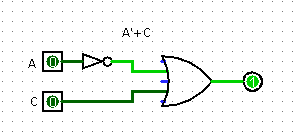
\includegraphics[width=0.8\textwidth]{assn/02/media/10b.png}
        \caption{Circuit Diagram of the Truth Table 10b in Logisim}
      \end{figure}
      % \clearpage

      \item
      \noindent
      $\displaystyle
      \left[
        \begin{array}{c c c|c}
          \textbf{A} & \textbf{B} & \textbf{C} & \textbf{f(A,B,C)} \\
          \hline
          0 & 0 & 0 & 1 \\
          0 & 0 & 1 & 0 \\
          0 & 1 & 0 & 0 \\
          0 & 1 & 1 & 1 \\
          1 & 0 & 0 & 1 \\
          1 & 0 & 1 & 1 \\
          1 & 1 & 0 & 1 \\
          1 & 1 & 1 & 1
        \end{array}
      \right]$

      \vspace{2em}
      \textbf{Answer:}
      \begin{Karnaughvuit}
        \maxterms{1,2}
        \minterms{0,3,4,5,6,7}
        \implicant{0}{4}{red}
        \implicant{3}{7}{green}
        \implicant{4}{6}{blue}
      \end{Karnaughvuit}

      DNF: $\overline{A}\overline{B}\overline{C} + A\overline{B}\overline{C} + \overline{A}BC + ABC + A\overline{B}\overline{C} + A\overline{B}C + ABC + AB\overline{C}$

      Minimal equation: $A + \overline{B}\overline{C} + BC$

      Show $\overline{A}\overline{B}\overline{C} + A\overline{B}\overline{C} + \overline{A}BC + ABC + A\overline{B}\overline{C} + A\overline{B}C + ABC + AB\overline{C} = A + \overline{B}\overline{C} + BC$
      \begin{align*}
        &\overline{A}\overline{B}\overline{C} + A\overline{B}\overline{C} + \overline{A}BC + ABC + A\overline{B}\overline{C} + A\overline{B}C + ABC + AB\overline{C}\\
        &=\overline{A}\overline{B}\overline{C} + A\overline{B}\overline{C} + \overline{A}BC + ABC + A\overline{B}C + AB\overline{C}\\
        &=\overline{A}\overline{B}\overline{C} + \overline{A}BC + A(\overline{B}\overline{C} + BC + \overline{B}C + B\overline{C})\\
        &=\overline{A}\overline{B}\overline{C} + \overline{A}BC + A(\overline{B} + \overline{C} + BC + \overline{B}C + B\overline{C})\\
        &=\overline{A}\overline{B}\overline{C} + \overline{A}BC + A(\overline{B} + \overline{C} + BC)\\
        &=\overline{A}\overline{B}\overline{C} + \overline{A}BC + A(\overline{B} + \overline{C} + C)\\
        &=\overline{A}\overline{B}\overline{C} + \overline{A}BC + A(\overline{B} + 1)\\
        &=\overline{A}\overline{B}\overline{C} + \overline{A}BC + A(1)\\
        &=\overline{A}(\overline{B}\overline{C} + BC) + A\\
        &=\overline{B}\overline{C} + BC + A\\
        &=A + \overline{B}\overline{C} + BC
      \end{align*}

      \begin{figure}[h]
        \centering
        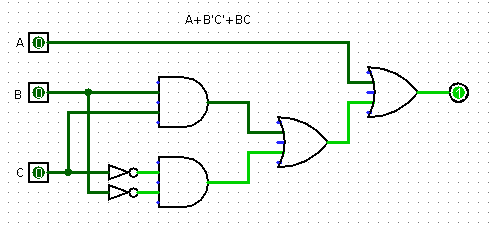
\includegraphics[width=0.8\textwidth]{assn/02/media/10c.png}
        \caption{Circuit Diagram of the Truth Table 10c in Logisim}
      \end{figure}

    \end{enumerate}

  \end{enumerate}

\end{document}
